\documentclass[pdftex,12pt,a4paper]{article}

\usepackage{graphicx}  
\usepackage[margin=2.5cm]{geometry}
\usepackage{breakcites}
\usepackage{indentfirst}
\usepackage{pgfgantt}
\usepackage{pdflscape}
\usepackage{float}
\usepackage{epsfig}
\usepackage{epstopdf}
\usepackage[cmex10]{amsmath}
\usepackage{stfloats}
\usepackage{multirow}
\usepackage{booktabs}
\usepackage{enumitem}
\usepackage{array,mathtools}
\usepackage{amssymb}
\newcommand*{\carry}[1][1]{\overset{#1}}
\newcolumntype{B}[1]{r*{#1}{@{\,}r}}


\renewcommand{\refname}{REFERENCES}
\linespread{1.3}

\usepackage{mathtools}
%\newcommand{\HRule}{\rule{\linewidth}{0.5mm}}
\thispagestyle{empty}
\begin{document}
\begin{titlepage}
\begin{center}
\textbf{}\\
\textbf{\Large{ISTANBUL TECHNICAL UNIVERSITY}}\\
\vspace{0.5cm}
\textbf{\Large{COMPUTER ENGINEERING DEPARTMENT}}\\
\vspace{2cm}
\textbf{\Large{BLG 242E\\ DIGITAL CIRCUITS LABORATORY\\ HOMEWORK REPORT}}\\
\vspace{2.8cm}
\begin{table}[ht]
\centering
\Large{
\begin{tabular}{lcl}
\textbf{HOMEWORK NO}  & : & 1 \\
\textbf{LAB SESSION}  & : & FRIDAY - 16.30 \\
\textbf{GROUP NO}  & : & 18 \\
\end{tabular}}
\end{table}
\vspace{1cm}
\textbf{\Large{GROUP MEMBERS:}}\\
\begin{table}[ht]
\centering
\Large{
\begin{tabular}{rcl}
150200916  & : & Denıs Iurıe Davıdoglu \\
150220770  & : & Onur Baylam \\
\end{tabular}}
\end{table}
\vspace{2.8cm}
\textbf{\Large{SPRING 2023}}

\end{center}

\end{titlepage}

\thispagestyle{empty}
\addtocontents{toc}{\contentsline {section}{\numberline {}FRONT COVER}{}}
\addtocontents{toc}{\contentsline {section}{\numberline {}CONTENTS}{}}
\setcounter{tocdepth}{4}
\tableofcontents
\clearpage

\setcounter{page}{1}

\section{INTRODUCTION}

In this homework, preliminary part revises basic digital circuits topics, such as 2's complement notation; minimization of logic functions using 
Karnaugh diagram and Quine-McCluskey method; implementing the same function with different logic components, such as universal NAND gates, multiplexer, decoder. In the experiment part, basic logic circuits are implemented and simulated in Verilog HDL, in the order of increasing complexity, with the final module being 16-Bit Adder-Subtractor.

\section{MATERIALS AND METHODS}



\subsection{Preliminary}

$ F_1 (a, b, c, d) = \cup_1 (0, 2, 6, 7, 8, 10, 11, 15) + \cup_{\phi} (4)$ \\
For the given function $F_1$, we apply given operations below:
\begin{enumerate}[label=\alph*)]
    \item Find its prime implicants using Karnaugh diagram.
\end{enumerate}
\begin{itemize}
    \item In order to obtain prime implicants of function \textbf{$F_1$}, we cluster all \textbf{true points} (1s) which are in the adjacent cells in the Karnaugh diagram into same group. Afterwards, we retain the constant literals and remove the changing ones. Moreover, if the truth value of a constant variable is \textbf{‘1’}, we use \textbf{true form} of that variable to write the relevant prime implicant. Otherwise, we use its \textbf{complement form}.\\

    \textbf{NOTE:} We assume \textbf{don't care terms ($\phi$)} to be \textbf{true} (1) to create larger groups.
\end{itemize}

\begin{figure}[H]
    \centering
        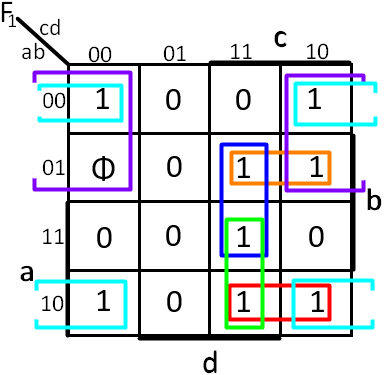
\includegraphics[width=0.5\textwidth]{map1.png}	
        \caption{Karnaugh map of the function  $F_1$}
        \label{fig1}
\end{figure}

\textbf{Set of all prime implicants:}\\

\begin{figure}[H]
    \centering
        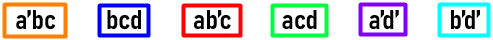
\includegraphics[width=0.5\textwidth]{primeimplicants.png}	
        \caption{Prime implicants of the function  $F_1$}
        \label{fig1}
\end{figure}

\begin{enumerate}[label=\alph*)]
  \setcounter{enumi}{1}
  \item Find its prime implicants using Quine-McCluskey method.

\begin{minipage}[t]{.3\textwidth} %
\begin{tabular}{|c|c|}
\hline
\multicolumn{2}{|c|}{Step 1} \\
\hline
Num & abcd \\
\hline
0 & 0000\checkmark \\
\hline
2 & 0010\checkmark \\
8 & 1000\checkmark \\
4 & 0100\checkmark \\
\hline
6 & 0110\checkmark \\
10 & 1010\checkmark \\
\hline
7 & 0111\checkmark \\
11 & 1011\checkmark \\
\hline
15 & 1111\checkmark \\
\hline
\end{tabular}
\end{minipage}%
\begin{minipage}[t]{.3\textwidth} %
\begin{tabular}{|c|c|}
\hline
\multicolumn{2}{|c|}{Step 2} \\
\hline
Num & abcd \\
\hline
2, 0 & 00-0\checkmark \\
8, 0 & -000\checkmark \\
4, 0 & 0-00\checkmark \\

\hline
6, 2 & 0-10\checkmark \\
10, 2 & -010\checkmark \\
10, 8 & 10-0\checkmark \\
6, 4 & 01-0\checkmark \\

\hline
7, 6 & 011- \\
11, 10 & 101- \\

\hline

15, 7 & -111 \\
15, 11 & 1-11 \\
\hline
\end{tabular}
\end{minipage}%
\begin{minipage}[t]{.3\textwidth} %
\begin{tabular}{|c|c|}
\hline
\multicolumn{2}{|c|}{Step 3} \\
\hline
Num & abcd \\
\hline
10, 8, 2, 0 & -0-0 \\
6, 4, 2, 0 &  0--0 \\
\hline

\end{tabular}
\end{minipage}

The rows without checkmark are unmatched and thus are the prime implicants: $\overline{a}bc, a\overline{b}c, bcd, acd, \overline{b}\overline{d}, \overline{a}\overline{d}.$ \\
  
\end{enumerate}

\begin{enumerate}[label=\alph*)]
  \setcounter{enumi}{2}
  \item Create prime implicant chart and find the expression with the minimum cost with 2 units of cost for each variable and 1 unit of cost for complement of a variable.\\
  
  First of all, we label each prime implicant with a symbol (letter). Afterwards, we calculate the cost of each prime implicant.

  \begin{figure}[H]
    \centering
        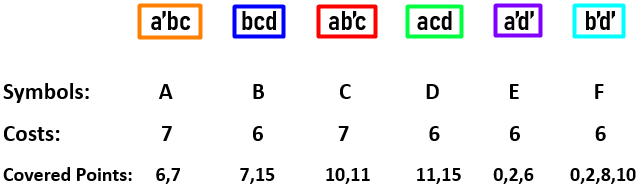
\includegraphics[width=0.7\textwidth]{implicantsymbol.png}	
        \caption{Prime implicants with symbols, costs and covered points}
        \label{fig1}
   \end{figure}

\textbf{NOTE:} Since there is no need to cover \textbf{don't care terms ($\phi$)}. We do not need to include them to the prime implicant chart.\\

\textbf{Prime Implicant Chart:}
    \begin{figure}[H]
    \centering
        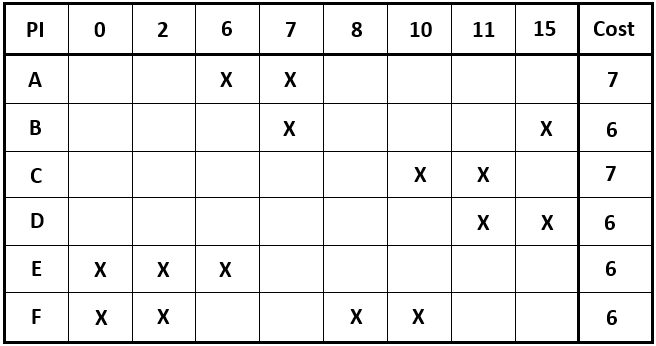
\includegraphics[width=0.7\textwidth]{chart1.png}	
        \caption{Prime implicant chart}
        \label{fig1}
   \end{figure}

   \textbf{Step 1:} In the prime implicant chart, \textbf{F} is an essential prime implicant which covers the distinguished point \textbf{8}. Therefore, we need to select prime implicant \textbf{F} to be able to cover point \textbf{8}.\\
   
   We mark F to indicate that it will be included to the minimal covering sum.
   \begin{figure}[H]
    \centering
        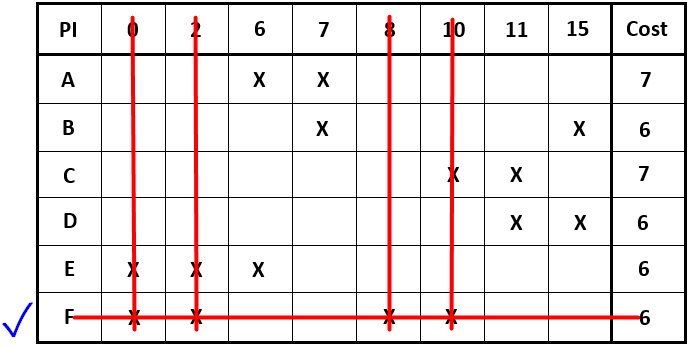
\includegraphics[width=0.7\textwidth]{chart2.png}	
        \caption{Prime implicant \textbf{F} is selected}
        \label{fig1}
   \end{figure}

   \textbf{The new form of the prime implicant chart:}
   \begin{figure}[H]
    \centering
        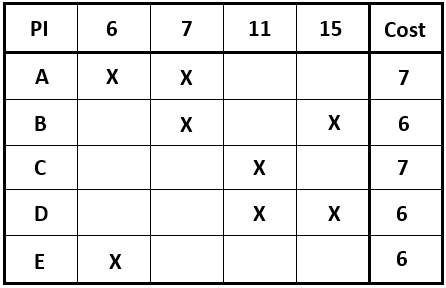
\includegraphics[width=0.6\textwidth]{chart3.png}	
        \caption{New form of the prime implicant chart}
        \label{fig1}
   \end{figure}

   \textbf{Step 2:} In the prime implicant chart, \textbf{D} covers \textbf{C} and the cost of \textbf{D} is smaller than the cost of \textbf{C}. So, we can remove \textbf{C} from the chart.

   \begin{figure}[H]
    \centering
        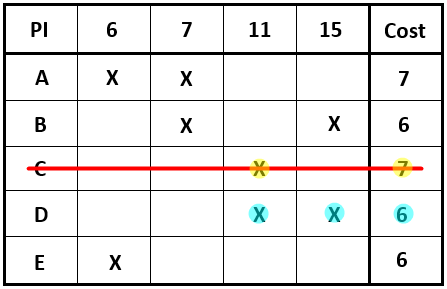
\includegraphics[width=0.6\textwidth]{chart4.png}	
        \caption{\textbf{C} is removed from the chart}
        \label{fig1}
   \end{figure}
    
   \textbf{The new form of the prime implicant chart:}
   \begin{figure}[H]
    \centering
        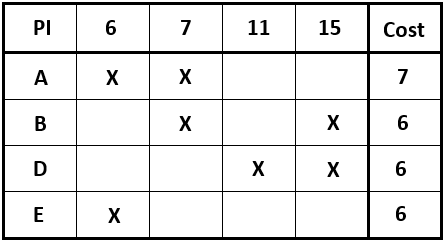
\includegraphics[width=0.6\textwidth]{chart5.png}	
        \caption{New form of the prime implicant chart}
        \label{fig1}
   \end{figure} 

   \textbf{Step 3:} In the new form of the chart, \textbf{D} is an essential prime implicant which covers the distinguished point \textbf{11}. Therefore, we select \textbf{D} and remove it from the chart.

   \begin{figure}[H]
    \centering
        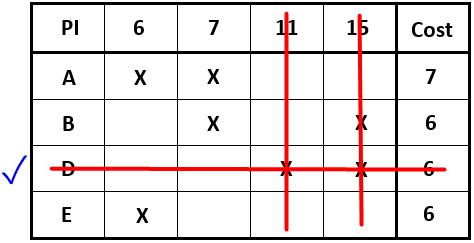
\includegraphics[width=0.6\textwidth]{chart6.png}	
        \caption{Prime implicant \textbf{D} is selected}
        \label{fig1}
   \end{figure}

   \textbf{The new form of the prime implicant chart:}
   \begin{figure}[H]
    \centering
        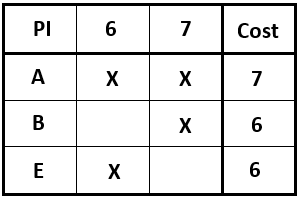
\includegraphics[width=0.5\textwidth]{chart7.png}	
        \caption{New form of the prime implicant chart}
        \label{fig1}
   \end{figure}

   \textbf{Step 4:} To cover all true points with minimum cost, we need to select prime implicant \textbf{A}. As a result, we select \textbf{A} and form our minimal covering sum.

   \begin{figure}[H]
    \centering
        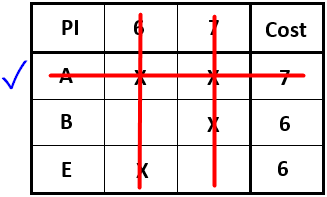
\includegraphics[width=0.5\textwidth]{chart8.png}	
        \caption{Prime implicant \textbf{A} is selected}
        \label{fig1}
   \end{figure}

   \textbf{Minimal Covering Sum:}
   \begin{figure}[H]
    \centering
        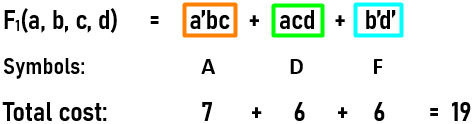
\includegraphics[width=0.6\textwidth]{chart9.png}	
        \caption{The expression with the minimum cost for function $F_1$}
        \label{fig1}
   \end{figure}
\end{enumerate}
    
\newpage

\begin{enumerate}[label=\alph*)]
  \setcounter{enumi}{3}
  \item Design and draw the lowest cost expression using NOT, AND, and OR gates.
	
  \begin{figure}[H]
    \centering
        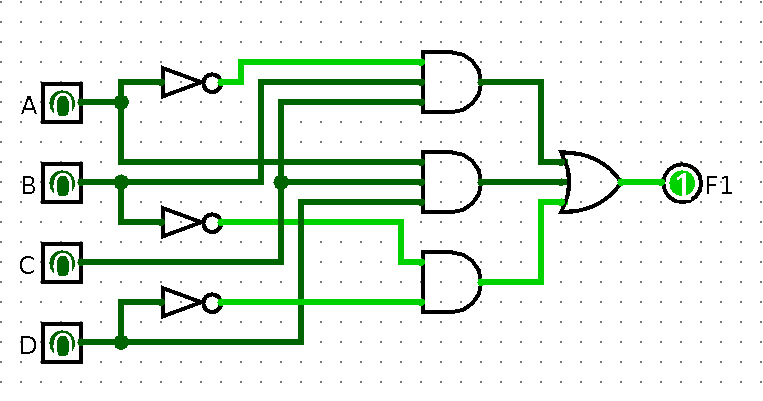
\includegraphics[width=0.9\textwidth]{Prem1AND_OR.png}	
        \label{fig1}
   \end{figure}
   


  \item Design and draw the lowest cost expression using only NAND gates.

  \begin{figure}[H]
    \centering
        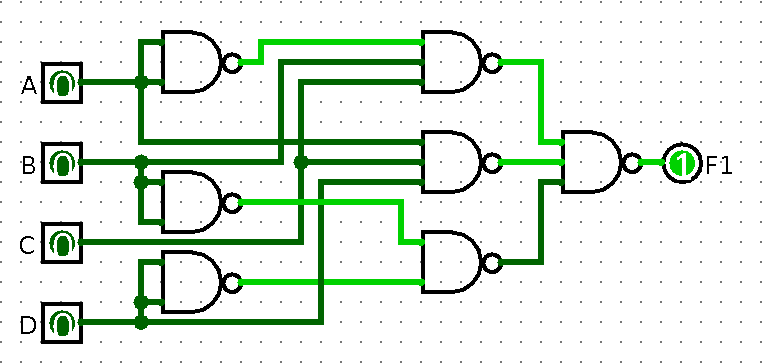
\includegraphics[width=0.9\textwidth]{Prem1NAND.png}	
        \label{fig1}
   \end{figure}

\newpage
  \item Design and draw the lowest cost expression using a single 8:1 Multiplexer, AND, OR and NOT gates.
	\begin{figure}[H]
    \centering
        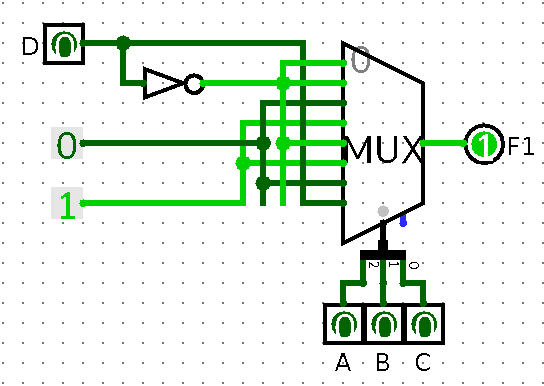
\includegraphics[width=0.7\textwidth]{Prem1MUX.png}	
        \label{fig1}
   \end{figure}	

\end{enumerate}	

\begin{enumerate}[label = \arabic*.]
\setcounter{enumi}{1}
\item Design and draw the functions $F_2$ and $F_3$ given using ONE single 3:8 decoder, 2-input OR gates.	

$F_2 (a, b, c) = \overline{a}bc + a\overline{b}c$, 
$F_3 (a, b, c) = ab\overline{c} + ab$
	\begin{figure}[H]
    \centering
        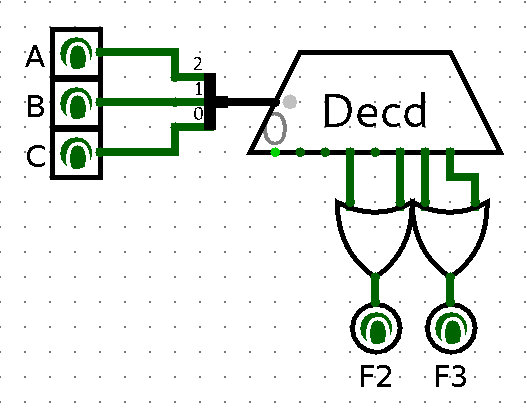
\includegraphics[width=0.6\textwidth]{Prem2.png}	
        \label{fig1}
   \end{figure}	

\newpage

\item
	\begin{itemize}
		\item Recall signed and unsigned addition for binary numbers in 2’s complement notation.
		\item Recall signed and unsigned subtraction for binary numbers in 2’s complement notation.
		
		In 2's complement notation, both addition and subtraction use the same table:
\begin{minipage}{1\textwidth}
\centering
\begin{tabular}{cc|cc}
    $a$ & $b$ & $sum$ & $carry$ \\
    \hline
    0 & 0 & 0 & 0 \\
    0 & 1 & 1 & 0 \\
    1 & 0 & 1 & 0 \\
    1 & 1 & 0 & 1 \\
  \end{tabular}
\end{minipage}

Addition is performed without any changes to the numbers, both for unsigned and signed. Only the most significant bit is interpreted differently, being reserved for sign in the signed representation, and used normally in the unsigned:

\begin{minipage}{0.5\textwidth}
  \centering
  \begin{equation*}
    \begin{array}{B3}
      0 & 0100 & 0 \carry 010 \\
      {} + 0 &                             0001 &                      1011 \\ \hline
      0 &                             0101 &                      1101 \\
    \end{array}
  \end{equation*}
\end{minipage}%
\begin{minipage}{0.5\textwidth}
  \centering
  \begin{equation*}
    \begin{array}{B3}
      \carry 0 & \carry 1\carry 1\carry 0\carry 0 & \carry 1\carry 0\carry 01 \\
      {} + 0 &                             1111 &                      1111 \\ \hline
      1 &                             1100 &                      1000 \\
    \end{array}
  \end{equation*}
\end{minipage}

Subtraction, on the other hand, firstly requires transforming a number into 2's complement, which is done by flipping the bits and adding one. For example, to compute $(01010011)_2 - (00000101)_2$, instead of performing subtraction, addition with the 2's complement of the subtrahend can be done: 

$(\overline{00000101})_2 + 1 = (11111010)_2 + 1 = (11111011)_2$


  \begin{equation*}
    \begin{array}{B3}
      \carry 0 & \carry 0\carry 1\carry 0 1 & 0\carry 0\carry 11 \\
      {} + 0 &                             1111 &                      1011 \\ \hline
      1 &                             0100 &                      1110 \\
    \end{array}
  \end{equation*}
The extra bit that arises after addition will be ignored and not counted as part of result; however, it can be used to interpret which number was bigger, if there was overflow or borrow, if the result can be represented, all depending on the type of operation and whether the numbers were signed or unsigned.
	
	\end{itemize}
\end{enumerate}


\newpage
\subsection{Experiment}
\begin{itemize}
    \item \textbf{Part 1: Simulation results of AND, OR, NOT, XOR, NAND, 8:1 Multiplexer and 3:8 Decoder modules}\\

    \textbf{AND Module Simulation Result:} This module operates as an AND gate.
    \begin{figure}[H]
    \centering
        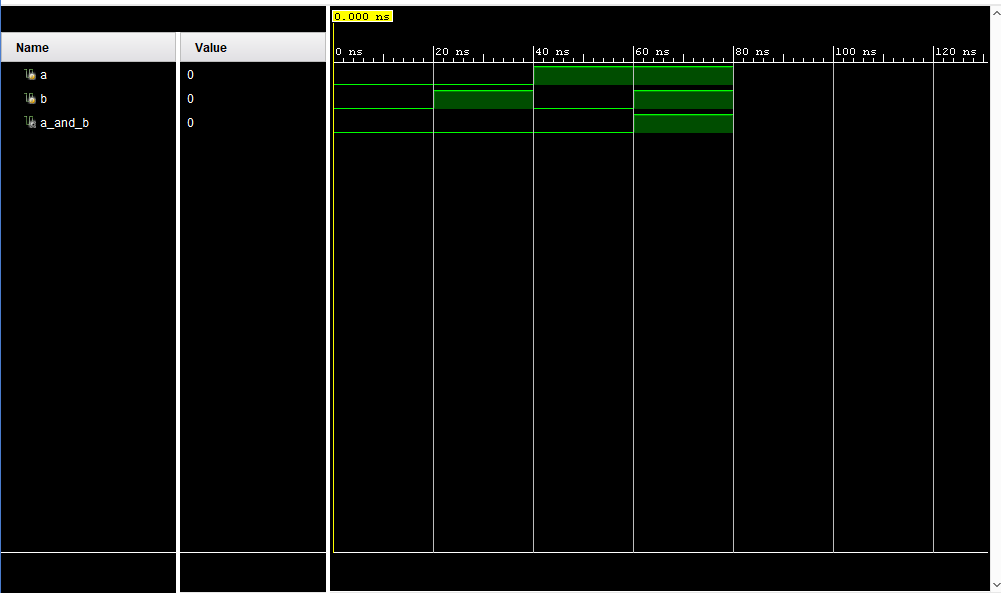
\includegraphics[width=0.9\textwidth]{AND.png}	
        \caption{AND module simulation result}
        \label{fig1}
   \end{figure}
\newpage
   \textbf{OR Module Simulation Result:} This module operates as an OR gate.
    \begin{figure}[H]
    \centering
        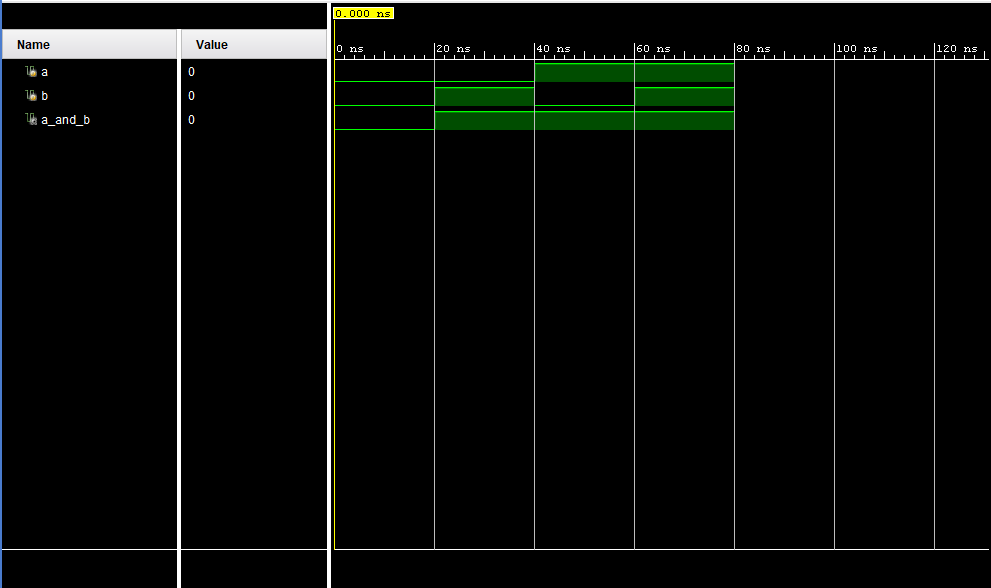
\includegraphics[width=0.9\textwidth]{OR.png}	
        \caption{OR module simulation result}
        \label{fig1}
   \end{figure}

   \textbf{NOT Module Simulation Result:} This module operates as a NOT gate.
    \begin{figure}[H]
    \centering
        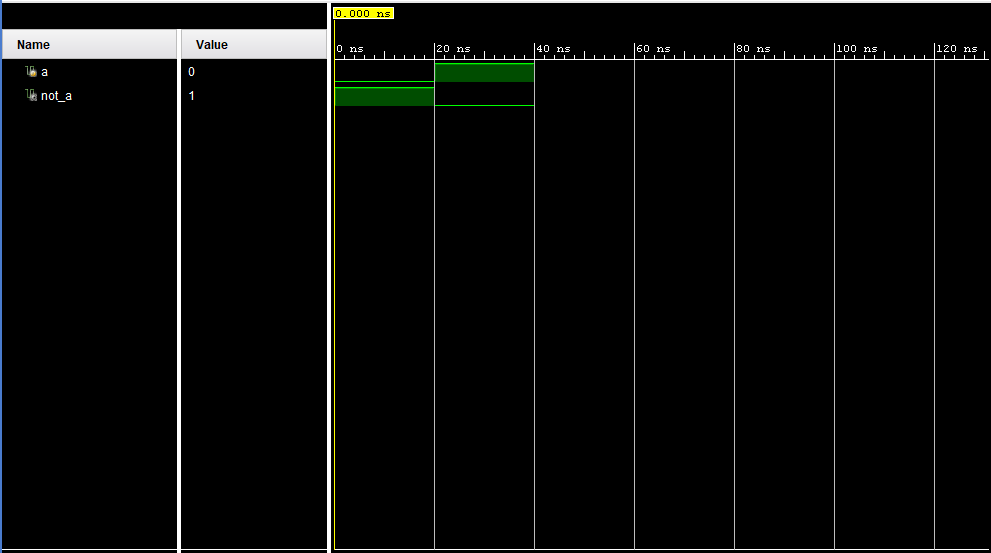
\includegraphics[width=0.9\textwidth]{NOT.png}	
        \caption{NOT module simulation result}
        \label{fig1}
   \end{figure}
\newpage
   \textbf{XOR Module Simulation Result:} This module operates as an XOR gate.
    \begin{figure}[H]
    \centering
        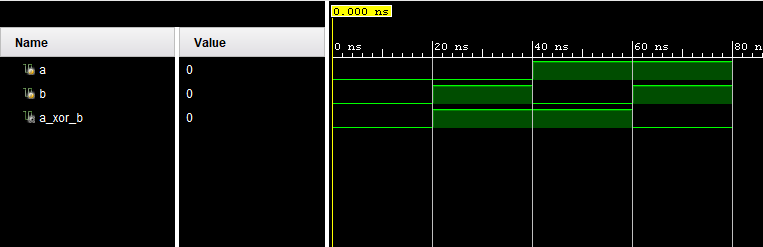
\includegraphics[width=0.9\textwidth]{XOR.png}	
        \caption{XOR module simulation result}
        \label{fig1}
   \end{figure}

   \textbf{NAND Module Simulation Result:} This module operates as a NAND gate.
    \begin{figure}[H]
    \centering
        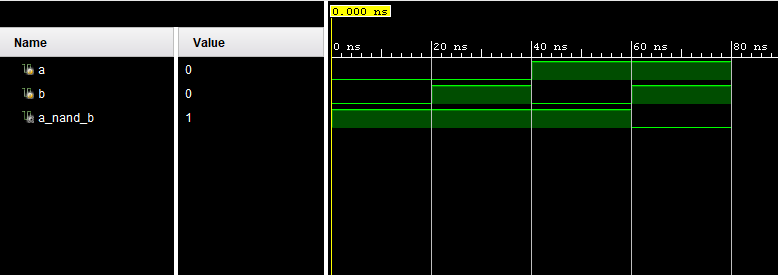
\includegraphics[width=0.9\textwidth]{NAND.png}	
        \caption{NAND module simulation result}
        \label{fig1}
   \end{figure}

   \textbf{8:1 Multiplexer Module Simulation Result:} This module operates as an 8:1 Multiplexer.
    \begin{figure}[H]
    \centering
        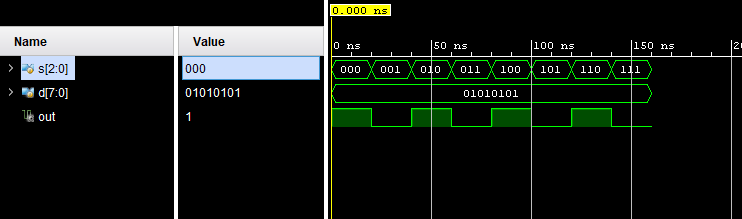
\includegraphics[width=0.9\textwidth]{MUX.png}	
        \caption{8:1 Multiplexer module simulation result}
        \label{fig1}
   \end{figure}
\newpage
   \textbf{3:8 Decoder Module Simulation Result:} This module operates as a 3:8 Decoder.
    \begin{figure}[H]
    \centering
        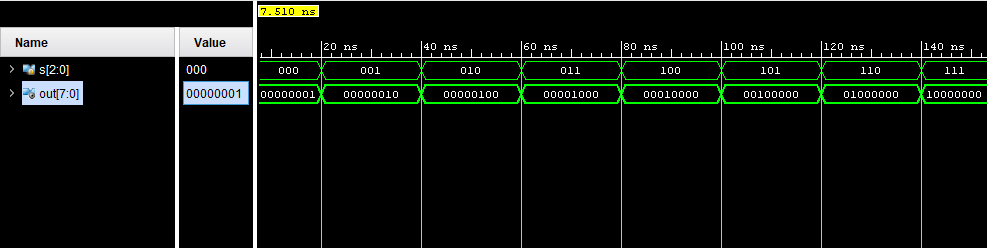
\includegraphics[width=0.9\textwidth]{Decoder.png}	
        \caption{3:8 Decoder module simulation result}
        \label{fig1}
   \end{figure}
\end{itemize}
\begin{itemize}
    \item \textbf{Part 2: Simulation result of $F_1$ in Preliminary 1.d.}\\
    Simulation result of the function $F_1$ designed in Preliminary 1.d. section using NOT, AND, and OR modules.
    \begin{figure}[H]
    \centering
        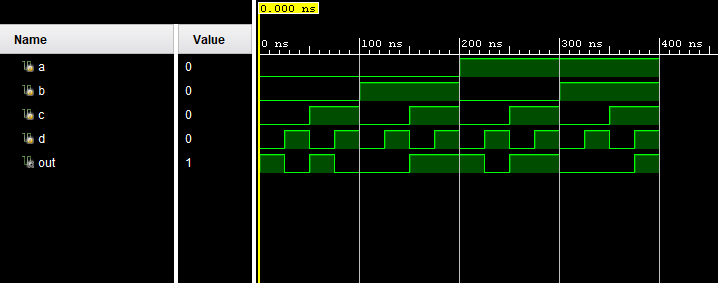
\includegraphics[width=0.9\textwidth]{1d.png}	
        \caption{Preliminary 1.d. $F_1$ simulation result}
        \label{fig1}
   \end{figure}
\end{itemize}
\newpage
\begin{itemize}
    \item \textbf{Part 3: Simulation result of $F_1$ in Preliminary 1.e.}\\
    Simulation result of the function $F_1$ designed in Preliminary 1.e. section using only NAND modules.
    \begin{figure}[H]
    \centering
        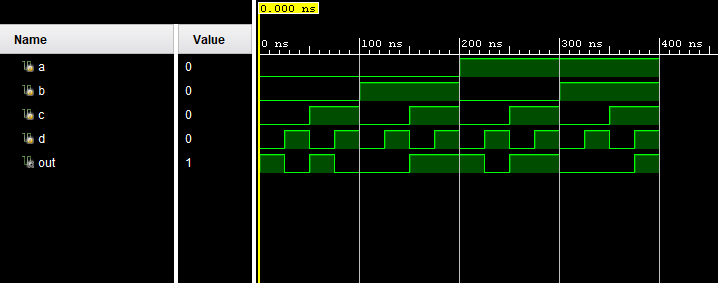
\includegraphics[width=0.9\textwidth]{1d.png}	
        \caption{Preliminary 1.e. $F_1$ simulation result}
        \label{fig1}
   \end{figure}
\end{itemize}
\begin{itemize}
    \item \textbf{Part 4: Simulation result of $F_1$ in Preliminary 1.f.}\\
    Simulation result of the function $F_1$ designed in Preliminary 1.f. section using a 8:1 multiplexer, AND, OR and NOT gates.
    \begin{figure}[H]
    \centering
        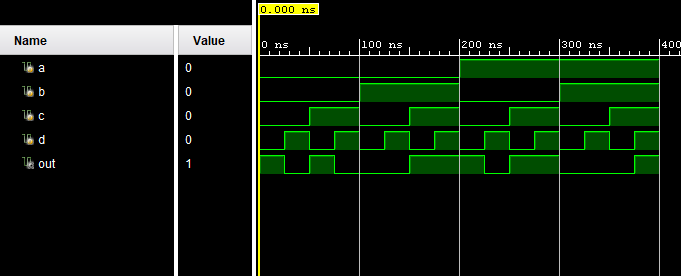
\includegraphics[width=0.9\textwidth]{1f.png}	
        \caption{Preliminary 1.f. $F_1$ simulation result}
        \label{fig1}
   \end{figure}
\end{itemize}
\newpage
\begin{itemize}
    \item \textbf{Part 5: Simulation results of $F_2$ and $F_3$ in Preliminary 2.}\\
    Simulation result of the function $F_2$ and $F_3$ designed in Preliminary 2 section using 3:8 Decoder and OR modules.
    \begin{figure}[H]
    \centering
        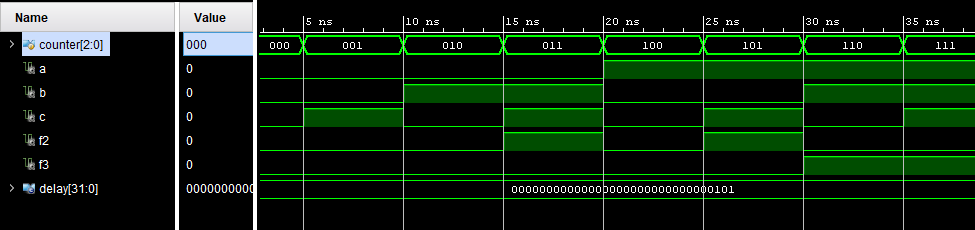
\includegraphics[width=0.9\textwidth]{part5.png}	
        \caption{Preliminary 2. $F_2$ and $F_3$ simulation result}
        \label{fig1}
   \end{figure}
\end{itemize}
\begin{itemize}
    \item \textbf{Part 6: Simulation result of 1-Bit Half Adder.}\\
    Simulation result of 1-Bit Half Adder using AND, OR, NOT, XOR modules.
    \begin{figure}[H]
    \centering
        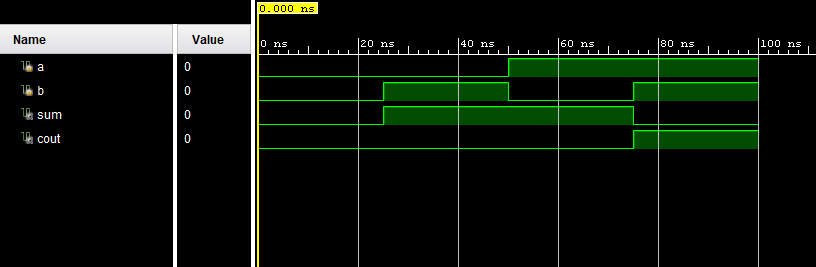
\includegraphics[width=0.9\textwidth]{halfadder.png}	
        \caption{1-Bit Half Adder Simulation Result}
        \label{fig1}
   \end{figure}
\end{itemize}
\newpage
\begin{itemize}
    \item \textbf{Part 7: Simulation result of 1-Bit Full Adder.}\\
    Simulation result of 1-Bit Full Adder using half adder and OR modules.
    \begin{figure}[H]
    \centering
        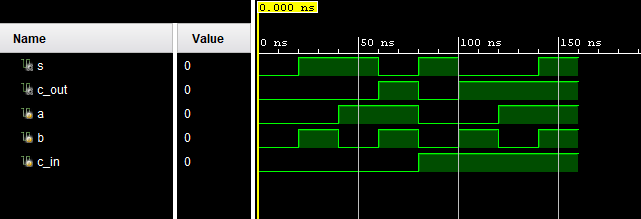
\includegraphics[width=0.9\textwidth]{fulladder.png}	
        \caption{1-Bit Full Adder Simulation Result}
        \label{fig1}
   \end{figure}
\end{itemize}
\begin{itemize}
    \item \textbf{Part 8: Simulation result of 4-Bit Full Adder.}\\
    Simulation result of 4-Bit Full Adder using 1-Bit Full Adder modules.
    \begin{figure}[H]
    \centering
        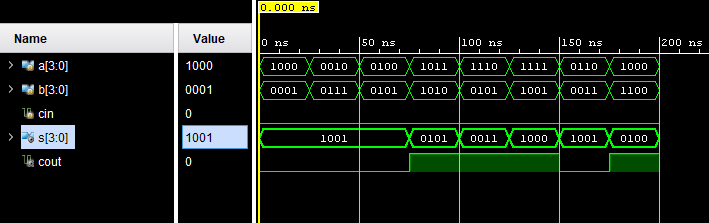
\includegraphics[width=0.9\textwidth]{fulladder4.png}	
        \caption{4-Bit Full Adder Simulation Result}
        \label{fig1}
   \end{figure}
\end{itemize}
\begin{itemize}
    \item \textbf{Part 9: Simulation result of 8-Bit Full Adder.}\\
    Simulation result of 8-Bit Full Adder by using 1-Bit Full Adder modules.
    \begin{figure}[H]
    \centering
        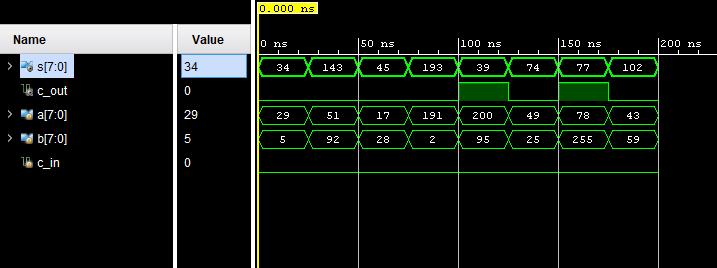
\includegraphics[width=0.9\textwidth]{fulladder8.png}	
        \caption{8-Bit Full Adder Simulation Result}
        \label{fig1}
   \end{figure}
\end{itemize}
\begin{itemize}
    \item \textbf{Part 10: Simulation result of 16-Bit Adder-Subtractor}\\
    Simulation result of 16-Bit Adder-Subtractor by using 8-Bit Full Adder and XOR modules.

    \textbf{NOTE:} The circuit operates on unsigned 16-bit binary numbers.
    \begin{figure}[H]
    \centering
        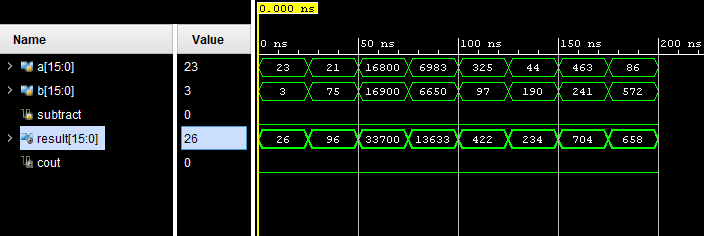
\includegraphics[width=0.9\textwidth]{addersub.png}	
        \caption{16-Bit Adder-Subtractor Simulation Result}
        \label{fig1}
   \end{figure}
\end{itemize}
\begin{itemize}
    \item \textbf{Part 11: Simulation result of the circuit which calculates B-2A}\\
    Simulation result of B-2A by using 16-Bit Adder-Subtractor, Adder, NOT, XOR, AND, and OR modules.

    \begin{figure}[H]
    \centering
        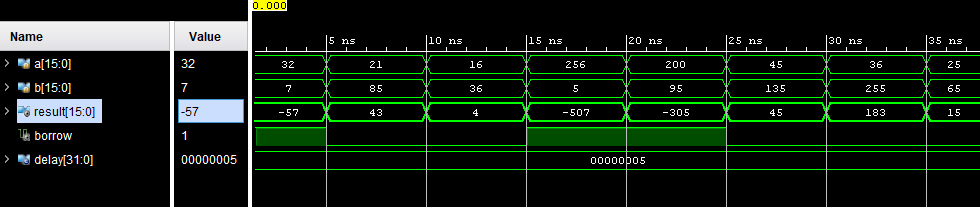
\includegraphics[width=0.9\textwidth]{part11.png}	
        \caption{Simulation result of B-2A calculator module}
        \label{fig1}
   \end{figure}
\end{itemize}


\section{CONCLUSION}
In this homework, we have applied our knowledge from the digital circuits course by deriving least cost expressions with human-friendly Karnaugh maps and a more algorithmic Quine-McCluskey method; facing the challenge to use only one kind of logic components, which happens in real life; learned to use Verilog HDL instead o Logisim for simulating circuits; built a fully working 16-bit adder-subtractor, whose functionality can be tracked down to the basic two-input gates. While using  Verilog HDL, simulating circuits and interpreting results was harder than designing the circuit in the first place because as the circuit gets more complex, the number of possible outcomes increases and one should be clever enough to provide proper tests with edge cases, instead of brute-forcing all input combinations. It is no surprise that the name Verilog is a portmanteau of the words "verification" and "logic". Although challenging with features unusual to most programming languages, it is very powerful for creating virtual hardware and verifying real devices. With the vast options for exporting the results of a simulation, such as exporting to waveform viewing programs, it dominates over Logisim or, even worse, truth table-generating websites. One disadvantage is that the circuit described is not available as a schematic. Nonetheless, we felt more like engineers as we designed and simulated digital circuits with this toolbox.

\newpage

\bibliographystyle{unsrt}

\end{document}

